\chapter{Software Development}

\section{Arduino Code}\label{sec:arduino_code}

We used an Arduino Uno for signal transmission. It already has its own 10-bit 0-5V ADC for analog signal transmission. We already made the necessary signal processing on the hardware side, our signal oscillates around 2.5V and has a range of 0-5V. We can start to read the signal using Arduino without any problem or any signal loss.


Before starting to measure the analog signal, we measured the reading speed using the following benchmark code in order to decide what sampling rate we should use:

\begin{lstlisting}[language=C++, caption=Analog Read Benchmark Code, label=lst:analog_read_benchmark]
void loop() {
    unsigned long start = micros();
    analogRead(A0);
    unsigned long end = micros();
    Serial.println(end - start);
}
\end{lstlisting}

The code reads the analog signal from pin A0 and prints the time taken to read the signal in microseconds. We used this code to measure the analog signal reading speed of the Arduino Uno. The average time taken to read the analog signal was 112$\mu$s. This means that the Arduino Uno can read the analog signal at a rate of 8.9kHz. This is more than enough for our project, as the maximum frequency of the signal we are trying to measure is 2kHz.

According to \textcite{Wikiedia-NyquistShannon2024}, Nyquist-Shannon Sampling Theorem says the minimum sampling rate should be twice the maximum frequency of the signal. So, we need a minimum sampling rate of 4kHz, but more is better.

\newpage
\thispagestyle{plain}

Arduino Uno can read the analog signal at a rate of 8.9kHz, which is more than enough for our project but for stability (because read speed vary around 108$\mu$s to 116$\mu$s according to our benchmarks), we decided to use a sampling rate of 8kHz (125$\mu$s, more than benchmark average). To achieve this, we used the following code:

\begin{lstlisting}[language=C++, caption=Arduino Code for 8kHz Sampling Rate, label=lst:arduino_code]
void loop() {
    unsigned long startedAt = micros();

    // Send the sensor value to the serial port
    int sensorValue = analogRead(analogPin);
    Serial.println(sensorValue);

    unsigned long endedAt = micros();
    unsigned long timeTook = endedAt - startedAt;

    // 125us = 8kHz sampling rate
    unsigned long timeRemaining = 125 - timeTook;

    // Wait for the remaining time
    // this approach will give us 8kHz sampling rate in theory
    // But in practice, it may not be exactly 8kHz 
    // but it is good enough for our purposes
    if (timeRemaining > 0) {
        delayMicroseconds(timeRemaining);
    }
}
\end{lstlisting}

This code reads the analog signal from pin A0, prints the signal value to the serial port, and waits for the remaining time to achieve an 8kHz sampling rate. This code will give us an 8kHz sampling rate in theory, but in practice, it may not be exactly 8kHz. However, it is good enough for our purposes.

\newpage
\thispagestyle{plain}

While this code prints the analog signal value to the serial port at 8kHz sampling rate, we used a Python script to read the serial port. Sometimes, Python cannot read the serial data correctly because this process is an asynchronous process. Maybe Arduino sends half of the data before Python is ready to read it. To prevent this, we can use starting and ending characters for the serial communication and keep a buffer in Python. We used the following code for this purpose:

\begin{lstlisting}[language=C++, caption=Arduino Code with Start and End Characters, label=lst:arduino_code_start_end]
const int analogPin = A0;

// Define the starting and ending characters 
// for the serial communication. 
// Sometimes python cannot read the serial data incorrectly. 
// To prevent this, we can use starting and ending characters.
const String startingChar = "S";
const String endingCar = "E";

void loop() {
    unsigned long startedAt = micros();

    int sensorValue = analogRead(analogPin);
    
    // Print the value with starting and ending characters
    Serial.print(startingChar);
    Serial.print(sensorValue);
    Serial.println(endingCar);

    // On serial port: 
    // SxxxxE -> S: Start, E: End, xxxx: Sensor Value
    // Example
    // S338E -> S: Start, E: End, 338: Sensor Value

    unsigned long endedAt = micros();
    unsigned long timeTook = endedAt - startedAt;

    // 125us = 8kHz sampling rate
    unsigned long timeRemaining = 125 - timeTook;

    // Wait for the remaining time
    // this approach will give us 8kHz sampling rate in theory
    // But in practice, it may not be exactly 8kHz 
    // but it is good enough for our purposes
    if (timeRemaining > 0) {
        delayMicroseconds(timeRemaining);
    }
}
\end{lstlisting}

This code prints the analog signal value to the serial port with starting and ending characters. This way, we can prevent Python from reading the serial data incorrectly.

\newpage
\thispagestyle{plain}

\section{Python Code}

We used Python to read the serial port, process the analog signal and show the real-time signal on a GUI. As we mentioned in Section \ref{sec:arduino_code}, Arduino Code, we used starting and ending characters for the serial communication. We used these characters to prevent Python from reading the serial data incorrectly. We used the following code to read the serial port:

\begin{lstlisting}[language=Python, caption=Python Code to Read Serial Port, label=lst:python_code_read_serial]
# Read data from serial port. Read Arduino code for more details
data_buffer = ""
while ser.in_waiting > 0:
    try:
        char = ser.read().decode("utf-8")
        data_buffer += char

        if "E" in data_buffer and "S" in data_buffer:
            try:
                start_index = data_buffer.index("S")
                end_index = data_buffer.index("E")
                value_str = data_buffer[start_index + 1 : end_index]
                if value_str.isdigit():
                    analog_value = int(value_str)

                    # Normalize and zero center because 
                    # most of the dsp functions 
                    # require zero centered data
                    normalized = (
                        (analog_value / 1024.0) * 5.0
                    ) - 2.5

                    # Append the normalized value to the list
                    # So that we can plot it later
                    analog_data.append(normalized)
                    time_data.append(time.time())

                    while time_data and (time_data[-1] - time_data[0] > 5):
                        time_data.popleft()
                        analog_data.popleft()
            except ValueError:
                pass
            data_buffer = ""

    except UnicodeDecodeError:
        data_buffer = ""
    except Exception:
        data_buffer = ""
\end{lstlisting}

\newpage
\thispagestyle{plain}

With this code, we read the serial port and process the analog signal. We normalized the analog signal to be zero-centered because most of the digital signal processing functions require zero-centered data. We also kept the last 5 seconds of the data in the list to plot it later.

While these codes are the most important parts of the software development, we also developed a GUI to show the real-time signal which we are not mentioning the code here. The GUI is developed using the tkinter and matplotlib library. You can always check the full code from the GitHub repository of the project, which is given in Appendix \ref{sec:appendix_a}.

\begin{figure}[h]
	\centering
	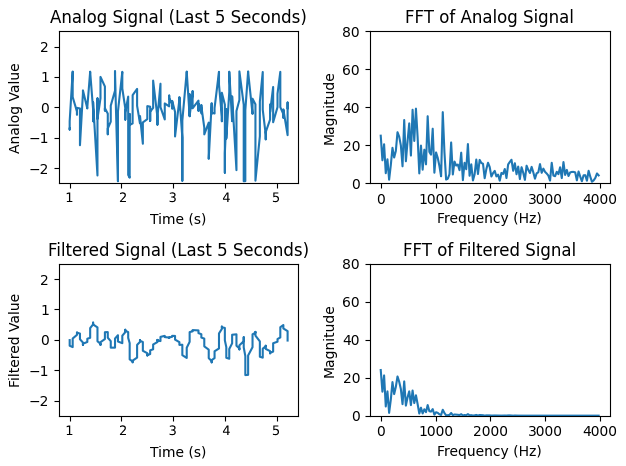
\includegraphics[width=0.8\textwidth]{assets/plots.png}
	\caption{GUI of the Project}
	\label{fig:gui}
\end{figure}

\begin{figure}[h]
	\centering
	\begin{minipage}{0.5\textwidth}
		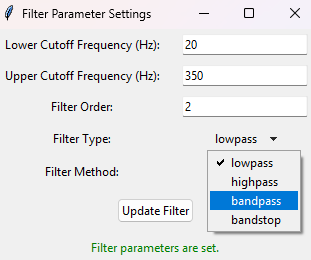
\includegraphics[width=0.9\textwidth , height=0.2\textheight]{assets/filter-type-selector.png}
		\caption{Filter Type Selector}
		\label{fig:gui-filter-type-selector}
	\end{minipage}%
	\begin{minipage}{0.5\textwidth}
		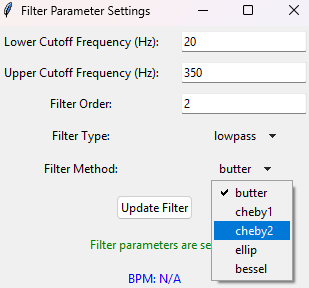
\includegraphics[width=0.9\textwidth , height=0.2\textheight]{assets/filter-method-selector.png}
		\caption{Filter Method Selector}
		\label{fig:gui-filter-method-selector}
	\end{minipage}
\end{figure}
